\documentclass{beamer}
\usetheme{AnnArbor}
\usepackage{graphicx}
\graphicspath{{pics/}}
\usepackage{amsmath}
\usepackage{amssymb}
\usepackage{framed}
\usepackage{tikz}
\usepackage[]{xcolor}
\usepackage[most]{tcolorbox}
\usepackage{pgfplots}
\pgfplotsset{compat=1.18}
\usepackage{blkarray}
\setbeamercolor{mycolorbox}{%
  bg=yellow!20,   % background color (20% yellow)
  fg=black      % foreground (text) color
}
\usefonttheme[onlymath]{serif}

\newtcolorbox{solutionblock}{
  colback=yellow!5,        % Background color: light yellow
  colframe=orange!80!black, % Frame color: dark orange
  title=Solution,
  fonttitle=\bfseries
}

\title{Introduction to Functions}
\author{Nithin}
\institute{}
\date{\today}
\begin{document}
\begin{frame}
  \titlepage
\end{frame}
\begin{frame}
  \tableofcontents
\end{frame}
\section{Slopes and Average Rate of Change}

% Slide: Motivation and Overview
\begin{frame}{Motivation: Why Study Change?}
  \begin{itemize}
    \item Calculus explores how quantities change and provides tools for modeling these changes.
    \item Functions link inputs ($x$) to outputs ($y=f(x)$); we investigate how $y$ varies as $x$ moves over an interval.
    \item Real-world example: Predicting economic indicators, modeling speeds, and more.
  \end{itemize}
\end{frame}

% Slide: Defining Average Rate of Change
\begin{frame}{Average Rate of Change}
  \begin{block}{Definition}
    For a function $f(x)$ on interval $[a,b]$, the \emph{average rate of change} is
    \[ 
      \frac{f(b)-f(a)}{b-a},
    \]
    which geometrically represents the slope of the secant line between $(a,f(a))$ and $(b,f(b))$.
  \end{block}
  \begin{itemize}
    \item Rise: $f(b)-f(a)$
    \item Run: $b-a$
    \item Secant line smooths out fluctuations; reports overall trend.
  \end{itemize}
\end{frame}

% Slide: Graphical Illustration
\begin{frame}{Graphical Illustration}
  \begin{columns}
    \column{0.6\textwidth}
      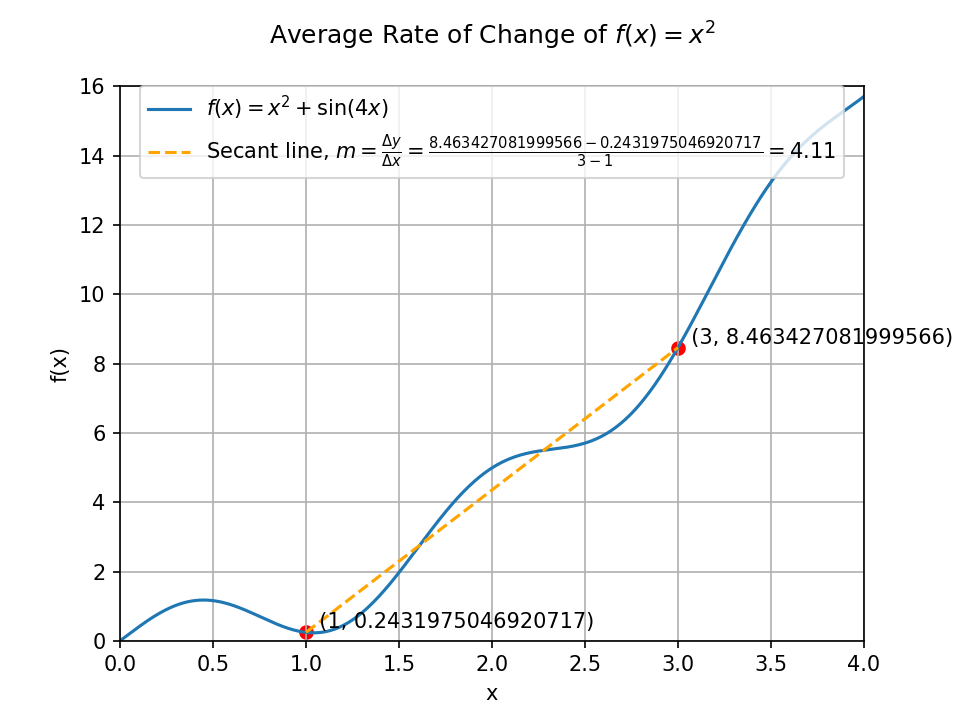
\includegraphics[width=\textwidth]{figures/avg_rate_of_change.png}
    \column{0.4\textwidth}
      \begin{itemize}
        \item Focus on interval $[1,3]$ on the curve $y=f(x)$.
        \item Secant line (in orange) joins $(1,f(1))$ and $(3,f(3))$.
        \item Its slope measures the average change in $y$ per unit change in $x$.
      \end{itemize}
  \end{columns}
\end{frame}

% Slide: Problem – Trivandrum to Chennai Average Speed
\begin{frame}{Example: Trivandrum to Chennai Journey}
  \begin{columns}
    \column{0.5\textwidth}
      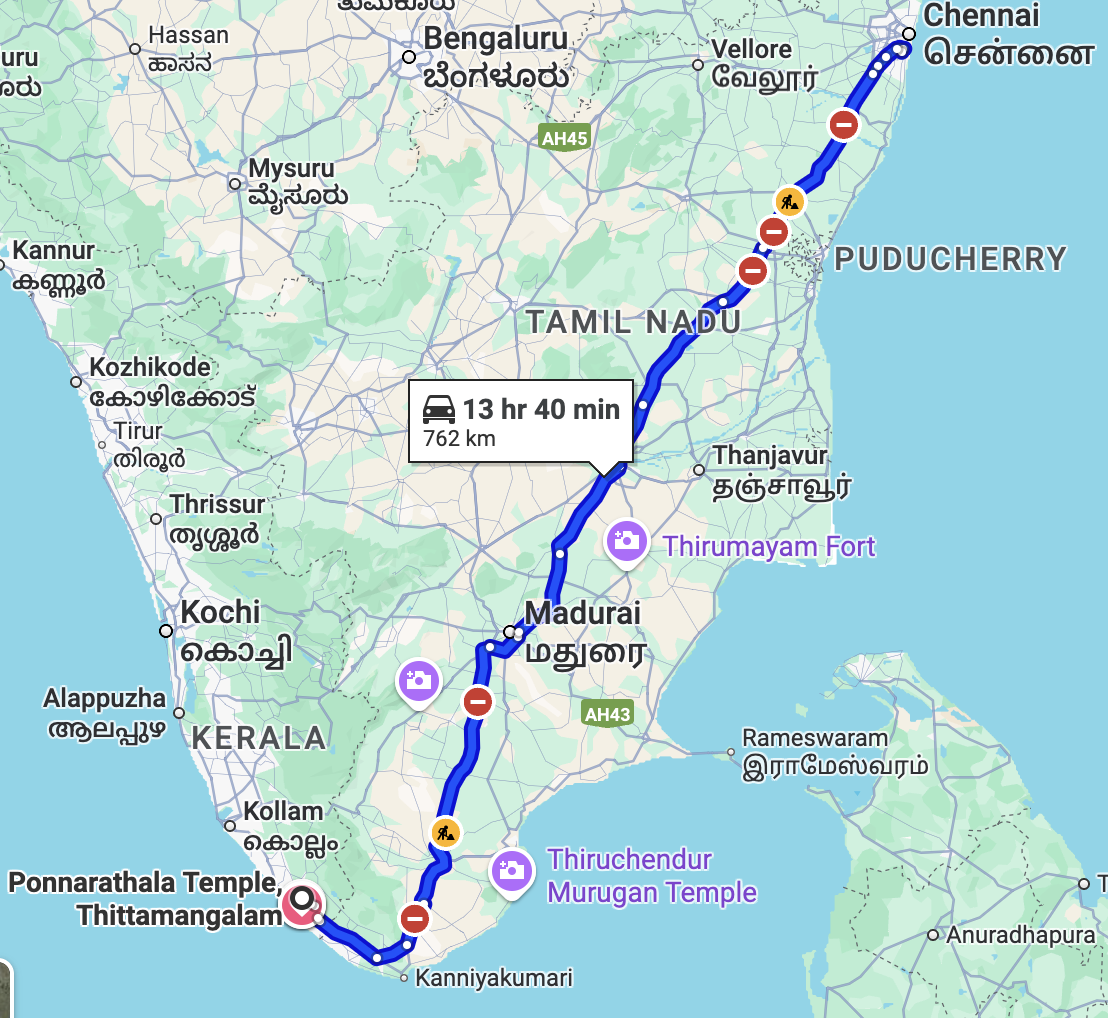
\includegraphics[width=\textwidth]{figures/trivandrum_chennai_map.png}
    \column{0.5\textwidth}
      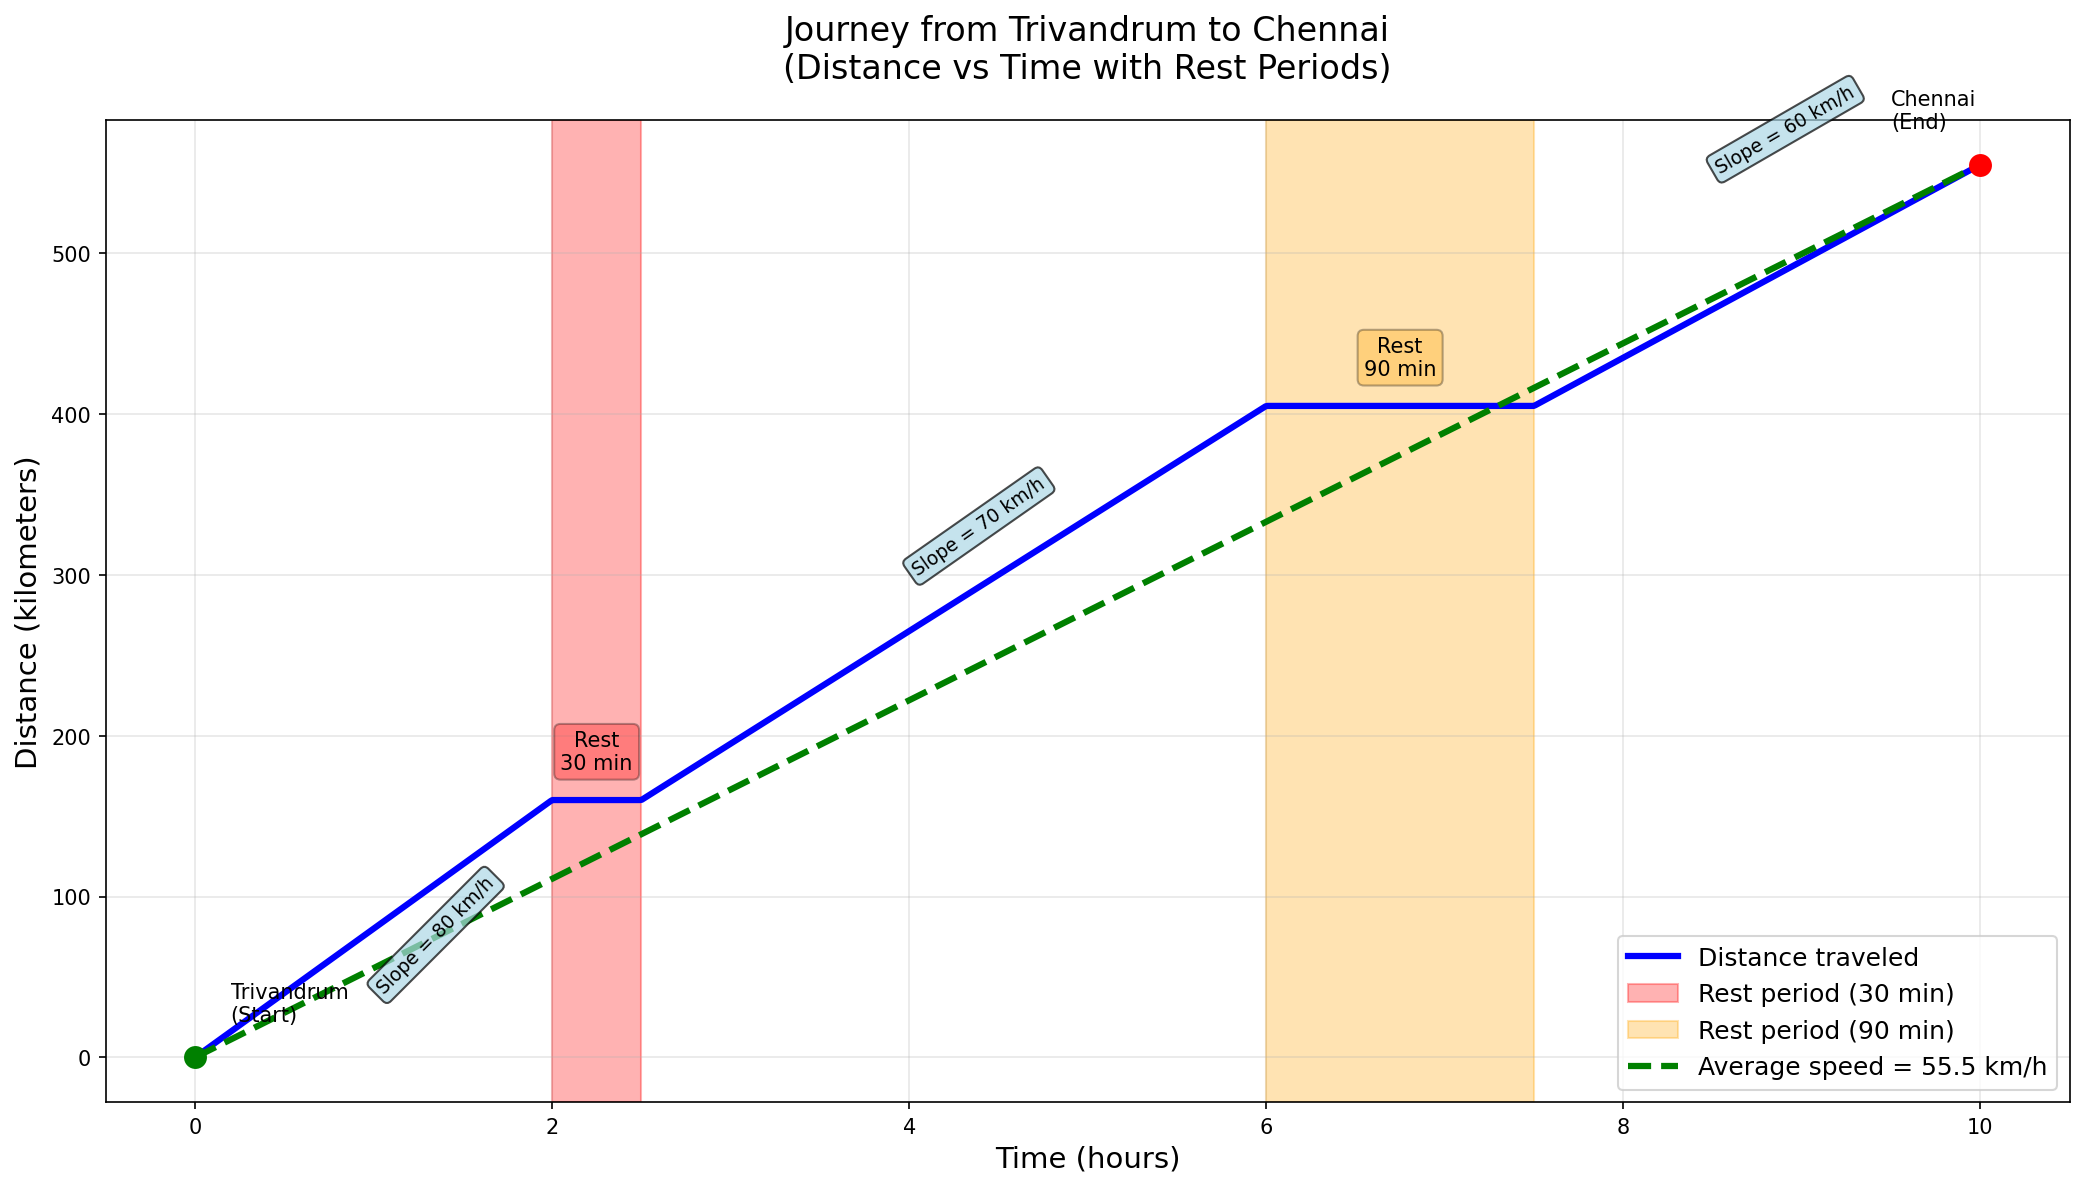
\includegraphics[width=\textwidth]{figures/trivandrum_chennai_journey.png}
  \end{columns}
  \vspace{1ex}
  \begin{itemize}
    \item Total distance: 762 km
    \item Total time (including stops): 15 hours
    \item Average speed: $\dfrac{762}{15}\approx50.8$ km/h
  \end{itemize}
  \begin{solutionblock}
    Average speed $=\dfrac{\text{distance}}{\text{time}}=\dfrac{762}{15}\approx50.8\text{ km/h}$.  
  This illustrates how the secant slope over an interval gives overall performance even with rest periods.
  \end{solutionblock}
\end{frame}

% Slide: Sensitivity to Rounding
\begin{frame}{Rounding and Accuracy}
  \begin{itemize}
    \item Distance measurements rounded to nearest kilometer introduce potential error.
    \item Small changes in endpoints can shift computed average speed above or below speed limit.
    \item Highlights importance of data precision in applications.
  \end{itemize}
\end{frame}

% Slide: Toward Instantaneous Rate of Change
\begin{frame}{Instantaneous Rate of Change}
  \begin{itemize}
    \item Instantaneous speed corresponds to slope of tangent line at a point.
    \item As secant interval shrinks ($b\to a$), average rate approaches derivative $f'(x)$.
    \item Next: Formalize tangent lines and derivatives.
  \end{itemize}
\end{frame}
\end{document}